\documentclass[Report1]{subfiles}

\begin{document}
\centerline{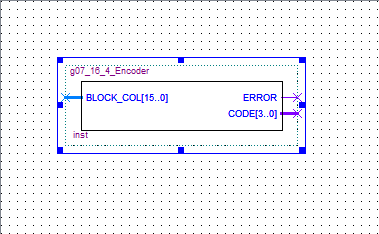
\includegraphics{encoder_schematic}}
\section{Circuit Explanation}
A 16:4 Encoder circuit has been created for this lab. The encoder circuit has a 16-bit input bus, a 4-bit output bus, and a single bit error output port. The purpose of the encoder is to get the number of low input bits from 16-bit input until the first high bit appears (i.e. the index of the lowest high input). The 4-bit output represents the number of low inputs until the first high input named, and is named CODE. The one single bit output is ERROR which is high when none of the input bit is high. Since we have 16-bit inputs, there are $2^{16}=65534$ possible combinations and CODE is in range of 0 to 15.
\end{document}